% This file was modified by Claude Sammut for ICML-2002 from the file
% made available by Pat Langley, Claude-Nicolas Fiechter, Mehmet Goker,
% and Cynthia Thompson for ICML-2K and by Andrea Danyluk for ICML-2002

% \documentstyle[icml2002,epsf]{article}
% If you rely on Latex2e packages, replace the above line with: 
\documentclass{article}
% For figures
\usepackage{graphicx} % more modern
%\usepackage{epsfig} % less modern
\usepackage{subfigure} 

% For citations
\usepackage{natbib}

% For algorithms
\usepackage{algorithm}
\usepackage{algorithmic}

% As of 2011, we use the hyperref package to produce hyperlinks in the
% resulting PDF.  If this breaks your system, please commend out the
% following usepackage line and replace \usepackage{icml2012} with
% \usepackage[nohyperref]{icml2012} above.
\usepackage{hyperref}

% Packages hyperref and algorithmic misbehave sometimes.  We can fix
% this with the following command.
\newcommand{\theHalgorithm}{\arabic{algorithm}}

% Employ the following version of the ``usepackage'' statement for
% submitting the draft version of the paper for review.  This will set
% the note in the first column to ``Under review.  Do not distribute.''
% \usepackage{icml2012} 
% Employ this version of the ``usepackage'' statement after the paper has
% been accepted, when creating the final version.  This will set the
% note in the first column to ``Appearing in''
\usepackage[accepted]{icml2012}

\begin{document} 

\twocolumn[
\icmltitle{Predicting Verb Relations between Subjects and Objects\\
			based on NELL Beliefs}

\icmlauthor{Guo Chen}{guoc@cs.cmu.edu}
\icmlauthor{Yilun Cui}{yilunc@cs.cmu.edu}
\icmladdress{Very Large Information Systems - SCS. Carnegie Mellon University, Pittsburgh PA.}

\vskip 0.3in
]

\section*{Abstract}

Relation prediction given the subject and the object is a new topic in the Never Ending Language Learning project. Our prediction mechanism uses large amounts of tuples from the \textbf{NELL SVO} corpus. We turned this task into a classification task having the verb as the label, and variants of the Naive Bayes classifier as our classification algorithm, all written in Map Reduce to accommodate for the data volume. We proposed strategies such as stemming, prior modifications. We also proposed a method to introduce categorical information into the Naive Bayes model via methods of smoothing. We evaluated our classifier and our techniques on different total possible labels.\\
\\
Experimental results comparing these strategies show our category approach significantly improve the accuracy of the Naive Bayes model.


\section{Introduction}

Never Ending Language Learner (NELL) is a learning system that extracts beliefs in the from of text online and tries to understand them. An important way to understand beliefs is to understand different entities and the relationship that ties entities together. Recently, NELL released a dataset that contains \emph{Subject}, \emph{Verb}, \emph{Object} tuples that it extracted from sentences online. We believe this dataset can be used to learn the relationship between entities, more specifically, we believe that the \emph{Verb} component reflects some notion of relationship.\\

To make this a learning task, we attempt to build a system that tries to understand the relationship between the two entities (\emph{Subject} and \emph{Object}) by trying to predict the \emph{Verb} that relates them.


Naive Bayes is a simple algorithm that is commonly used to solve text classification problems. Although there are other algorithms like Support Vector Machines which others have shown to preform better than Naive Bayes, the Naive Bayes algorithm scales well because probability calculations involves doing a series sums that can be done in parallel, this is favoured on large datasets. In a Bag of Words model, words are used as features and their word frequency is used as their values. To predict a label $L$ with given words $w$, the optima we try to arrive at is the following:

\begin{equation}
	\hat{L} = \arg\max_L P(L|w) = \arg\max_L P(L)P(w|L)
\end{equation}

\begin{equation}
	\hat{L} = \arg\max_L P(L) \prod_i{P(w_i|L)}
\end{equation}

When calculating the \emph{maximum likelihood estimator} by simply taking the product of the probabilities given the counts, we can observe that if any word count is zero, the posterior probability immediately becomes zero. There are many ways to smooth the probabilities such that none of the probabilities will be zero. This is calculating the \emph{maximum a posteriori estimator}, it essentially applies some pre-conceived prior assumption on the probabilities that is not present in the count of the words itself.
\section{Related Works}

Dumais \emph{et al.} \cite{dumais2000hierarchical}
\section{Dataset, Features, Labels}

The goal of our work is to find the verb relationship between a subject entity and an object entity. Hence to turn this into a classification task, verbs become labels. Subject, objects and their related attributes become features for classification.\\
\\
We used two different datasets for this classification task. Our ultimate goal is to classify the belief instances that we find in the \textbf{NELL SVO} dataset. This dataset contains ~220 million \emph{Subject Verb Object Count} tuples that have been mined by NELL. However we use another dataset: \textbf{NELL RTW} formalized dataset to give us metadata over the subjects and objects in the \textbf{NELL SVO} dataset. This dataset provides similar information in the form of \emph{Entity Relation Value} however, it provides hierarchical categories for each of the entities and values.\\
\\
The same belief in the two different datasets are represented differently:\\
In the SVO dataset:\\
\emph{cat eat fish}\\
In the RTW dataset:\\
\emph{concept:animal:cat concept:animalseatfood concept:food:fish}\\
\\
We plan to use the categorical data from the \textbf{NELL RTW} dataset as supplementary features for subject and object, giving additional information for classification.\\ We can project the entities in the \textbf{NELL SVO} dataset onto the \textbf{NELL RTW} dataset to find what the categories for each individual subject and object are.\\
\section{Methods}

\subsection{Naive Bayes}
% mention prior

The problem can be defined as a text classification problem with the verbs as labels and the subject and object as features. For each SVO document, the number of features is fixed as two. According to the Naive Bayes conditional independency assumption, given the subject s and the object o, the Naive Bayes formula to predict verb $v$ is provided as below.

\begin{equation}
	\hat{v} = \arg\max_v P(v|so) = \arg\max_v P(v)P(s|v)P(o|v)
\end{equation}

One thing we notice here is that the subject and the object are not symmetric. "Cat eat fish" and "Fish eat cat" should not be considered equal. Based on this intuition, we have two different subject and 

However, there exist duplicated features with different labels. For example, a "cat" can eat "fish", and can also like a "fish". As a classifier, Naive Bayes only gives the label with the highest conditional probability. It doesn't produce multi labels results for a given input document. In our experiments, when the system make a prediction that is one of the correct labels, there will be one "true positive" and all other possible correct answers will be marked as "false negative".

\subsection{Scalability}

Conventional Naive Bayes implementations stores a structure the size of \\
\\
$|Features| * |Label|$ \\
\\
in memory. In our case, this would be a \\
\\
$(|Subject\_Categories|+|Unique\_Subject|\\+|Object\_Categories|+|Object\_Subject|) * |Verbs|$ \\

sized structure. This is unfeasible for the amount of data we are working with. To deal with such a large volume of data we proposed a Naive Bayes algorithm in MapReduce implemented in Hadoop. This method of Naive Bayes is similar to Streaming Naive Bayes and does not require large global structures to be kept.\\
\\
At a high level, this requires going over the data 4 times. Once to count the number of occurrences of each verb. Once to count the number of occurrences of each Subject, Object and their categorical counts. Once to train. Once to test and evaluate the results. At the end of each phase, we store some small statistics into the context of our map and reduce jobs such as the number of unique subjects, objects, ontology for the next task.\\
\\
We only need to transform counts into conditional probabilities in the testing phase, since conditional probabilities are only needed for each test example. We can do a map emitting $<$Subject\/Object, [TestNum, test\_counts, train\_counts]$>$. This way we can parallelize to the full extent by putting all necessary information to calculate conditional probabilities in the reducer for a given Subject or Object.

This implementation scales well with the task because there are a lot of different possible subjects and objects. Since almost every map phase emits the subject or object as the key, the problem can easily be parallelized. The limit is not reached until the number of reducers equals the number of unique keys.

\subsection{Stemming}

The dataset from SVO tuples are parsed from sentences and not stemmed. Stemming can help to merge different tuples and reduce both feature set size and label set size. However, considering the database for ontology contains unstemmed words, we can't stem the subject and object words in the data file because that stemming will increase the ontology matching failure rate.

Despite of that, verbs can be stemmed to reduce the possible label set size. Stemmed verbs can cannonicalize verbs that actually mean the same thing but are in different tense, for example \emph{provides} vs. \emph{provided}. This can reduce number of labels, prediction error, and also the size of the intermediate data. We used a simple \emph{Porter Stemmer} for this task.
% left to Yilun

\subsection{Smoothing}

Considering the sparsity of language models, the \emph{Maximum-likelihood Estimator} version of Naive Bayes would likely result in a posterior probability of zero. A Dirichlet prior is often used. The Dirichlet prior pulls the features to a uniform distribution at a certain strength according to parameter $\alpha$. In many cases, as a simplification, plus one smoothing is used as a simplified Dirichlet prior with $\alpha=1$.

\subsection{Categorical Smoothing}

\begin{figure}[ht]
\vskip 0.2in
\begin{center}
\centerline{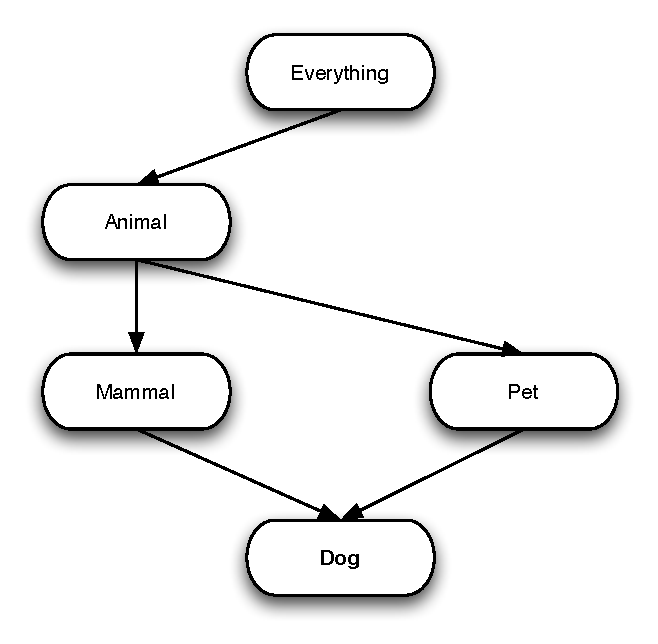
\includegraphics[width=\columnwidth]{dog}}
\caption{Categories for Dog}
\label{fig-dog-category-example}
\end{center}
\vskip -0.2in
\end{figure}

As mentioned before, NELL has a knowledge base with ontology information for many known entities. Usually more than one categories are provided for nouns. For example, a dog is a mammal, an animal, an everything and a pet. Some of the categories have containing relations. For the ``dog" example, we can describe the category relation as figure \ref{fig-dog-category-example}. As is shown in the figure, some categories like "mammal" are very close to the entity thus describe some attributes of the entity while others like "everything" are very faraway and thus not informative. In our observations, one degree parent categories are usually more helpful.

% \begin{figure}[ht]
% \vskip 0.2in
% \begin{center}
% \centerline{\includegraphics[width=\columnwidth]{icml_numpapers}}
% \caption{Historical locations and number of accepted papers for International
%   Machine Learning Conferences (ICML 1993 -- ICML 2008) and
%   International Workshops on Machine Learning (ML 1988 -- ML
%   1992). At the time this figure was produced, the number of
%   accepted papers for ICML 2008 was unknown and instead estimated.}
% \label{fig-dog-category-example}
% \end{center}
% \vskip -0.2in
% \end{figure}

In order to use the category information in the Naive Bayes model, we considered two approaches. One naive approach is to add category counts as independent features. In this way we increase the number of features for each document to above 4. However, this implementation heavily violates the strong dependent nature of these features. If a ``dog" is in the feature set, ``mammal" and ``pet" must also be in the feature set. But ``dog'', ``mammal'', and ``pet'' are highly correlated in reality. This means the model will have very high bias to begin with and probably will not work well.

Instead, we propose another approach, which is also our core contribution to this work. We introduce \emph{categorical smoothing}.\\

Recall with Laplace smoothing, we can say that we assume each word appears in each label approximately $\frac{1}{|w|}$ times with $\alpha = 1$.\\

\begin{equation}
	P(w|L) = \frac{Count(w|L)+\alpha}{Count(L)+\alpha |w|}
\end{equation}

With categorical smoothing, we know that the word is a member of a given category, thus its category can represent this word, so we assume that they appear $\frac{category(w)}{|categories|}$ of times. 

\begin{equation}
	P(w|L) = \frac{Count(w|L)+\alpha Count(category(w))}{Count(L)+\alpha \sum_i(category(i))}
\end{equation}

This method of smoothing takes independence of what the actual label is. It is a way to differentiate  where the different categories subjects and objects come from. Beliefs within the same category will not be effected by this type of smoothing because the weights applied are the same and hence only $Count(w|L)$ differentiates, but beliefs from different categories will be heavily influenced by this smoothing.

\subsection{Label Set}

As mentioned earlier, our label set is \emph{Verbs} that relate the subject and the object. There is non trivial number of verbs that can relate subjects and objects, hence the possible label space we expect to label is also quite large. We will do classification with controlled numbers of verbs/labels. Though we do expect that as the number of labels grow, the variance of the data will grow and that our classifiers will naturally become not as accurate.

\subsection{Evaluation and Metric}

We use NELL beliefs as labeled true data for training and testing. $10\%$ data is held out for test purpose and the other $90\%$ is training set. Cross validation could be a more useful technique but we don't intend to use it because it will require repetitive runs over the data and will be very computationally costly.

As a single-label prediction problem, we use precision as the metric to evaluate the classifier. According to the definition of precision,

\begin{equation}
	p = \frac{number_{truePositive}}{number_{truePositive} + number_{falsePositive}}
\end{equation}

Besides, different verbs for the same pair of subject and object are considered as different test cases. Since our system always predict one verb for a given subject-object pair, we always lose precision and recall on multi-label cases. Actually, considering it's a single-label prediction on a multi-label dataset, the precision is always equal to the recall.





\section{Experiment}

\subsection{Experimental Implementation}

Conventional Naive Bayes implementations stores a structure the size of \\
\\
$|Features| * |Label|$ \\
\\
in memory. In our classification case, this would be a \\
\\
$(|Subject\_Categories|+|Unique\_Subject|\\+|Object\_Categories|+|Object\_Subject|) * |Verbs|$ \\

sized structure. This is unfeasible for the amount of data we are working with. To deal with such a large volume of data we proposed a Naive Bayes algorithm in MapReduce implemented in Hadoop. This method of Naive Bayes is similar to Streaming Naive Bayes and does not require large global structures to be kept.\\
\\
At a high level, this requires going over the data 4 times. Once to count the number of occurrences of each verb. Once to count the number of occurrences of each Subject, Object and their categorical counts. Once to train. Once to test and evaluate the results. At the end of each phase, we store some small statistics into the context of our map and reduce jobs such as the number of unique subjects, objects, ontology for the next task.\\
\\
We only need to transform counts into conditional probabilities in the testing phase, since conditional probabilities are only needed for each test example. We can do a map emitting $<$Subject\/Object, [TestNum, test\_counts, train\_counts]$>$. This way we can parallelize to the full extent by putting all necessary information to calculate conditional probabilities in the reducer for a given Subject or Object. 

\subsection{Result Comparison}

\subsubsection{Comparison between categorical smoothing and Laplace smoothing}

\begin{table}[t]
\caption{Precision Comparison between categorical smoothing and Laplace smoothing}
\label{tab-smoothing-comparison}
\vskip 0.15in
\begin{center}
\begin{small}
\begin{sc}
\begin{tabular}{l|cc|c}
\hline
\abovespace\belowspace
Data set & Laplace & categorical & improvement \\
\hline
\abovespace
Top 1k set & 0.5906 & 0.8764 & 0.2858 \\
\belowspace
Lower 1k set & 0.6455 & 0.8128 & 0.1673 \\
\hline
\end{tabular}
\end{sc}
\end{small}
\end{center}
\vskip -0.1in
\end{table}

We use two different verb sets to compare the effect of categorical smoothing and Laplace smoothing. One set is the top 1000 most frequent unstemmed verbs in the SVO tuple corpus, the other lower 1000 set is the 10001st to 11000th most frequent unstemmed verbs in the SVO tuple corpus. The top 1000 set contains 538 unique stemmed verbs while the lower 1000 set contains 935 unique stemmed verbs. However, the number of examples in training and testing set are quite different. The top 1000 set has about 206k testing examples while the lower 1000 set has 18.9k testing examples. The numbers of training set have the same proportion.

From the comparison result in \ref{tab-smoothing-comparison}, we see that categorical smoothing provides a significant improvement on the precision on both datasets. It improves the precision on top 1000 set for 0.2858 and lower 1000 set for 0.1673 respectively. We also observe that the improvement of categorical smoothing is more significant on the top 1000 set than on the lower 1000 set.

\subsection{Comparison between Unigram Prior and Uniform Prior}

\begin{table}[t]
\caption{Precision Comparison between Unigram Prior and Uniform Prior}
\label{tab-prior-comparison}
\vskip 0.15in
\begin{center}
\begin{small}
\begin{sc}
\begin{tabular}{l|cc}
\hline
\abovespace \belowspace
Data set & Top 100 set & Lower 100 set \\
\hline
\abovespace
unigram prior & 0.8603 & 0.6376 \\
\belowspace
uniform prior & 0.9314 & 0.7784 \\
\hline
\abovespace
\belowspace
Difference & 0.0711 & 0.1408 \\
\hline
\end{tabular}
\end{sc}
\end{small}
\end{center}
\vskip -0.1in
\end{table}

\subsection{Smoothing Parameter}

\begin{figure}[ht]
\vskip 0.2in
\begin{center}
\centerline{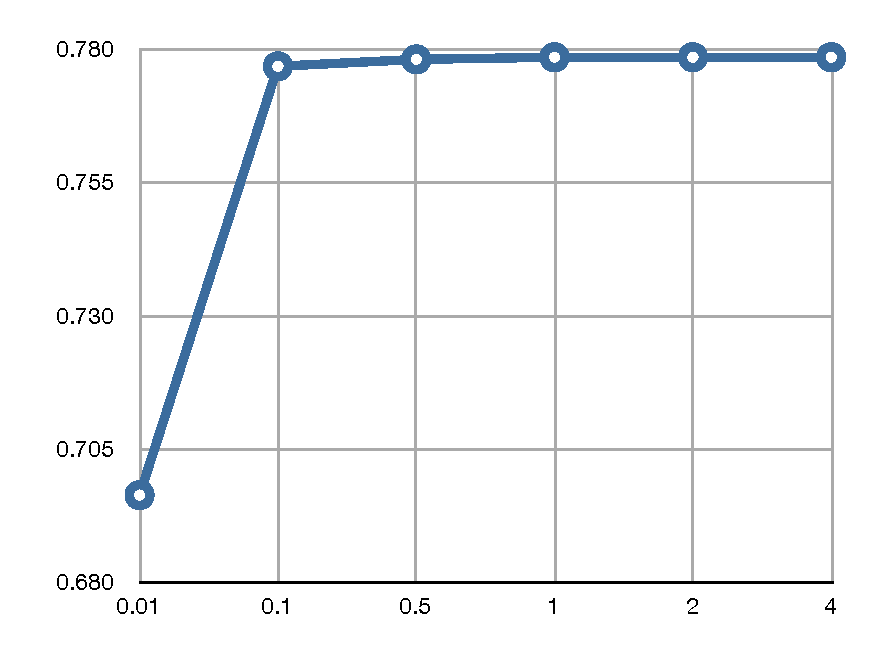
\includegraphics[width=\columnwidth]{pvsalpha}}
\caption{Precision vs. Smoothing parameter in Categorical Smoothing}
\label{fig-p-vs-alpha}
\end{center}
\vskip -0.2in
\end{figure}

We tuned the smoothing parameter $\alpha$ manually with several different values. When $\alpha$ is set to one, it is similar to Laplace smoothing but works on categorical counts instead of global vocabulary size. When $\alpha$ gets larger, the effect of category information is enlarged. From Figure \ref{fig-p-vs-alpha}, we find that when $\alpha$ is extreme small, the precision is decreased. When alpha increases, the precision generally increase, however, when alpha is larger than one, the precision is fixed on 0.7784 and never increases no matter how large it is set to.

We tried $\alpha=0$, and the experiment didn't success because of the zero probability product doesn't make sense. We tried to remove conditional probability of words and keep only the category based probability, but we got only a 0.0188 precision which is like random guess. We also had controlled experiments with Laplace smoothing with $\alpha=1$ and got the precision 0.6074, which is much lower than any alpha settings in categorical smoothing. 




\section{Conclusion}

The Naive Bayes model works very well on verb prediction task on NELL ontology information and SVO dataset. The dataset has a large number of verbs and hundreds of millions of SVO documents. We use two feature Naive Bayes on Hadoop to predict verbs within a given label set. 

Instead of Laplace smoothing, we use categorical smoothing to introduce category information of the features into the conditional probability estimators, and into Naive Bayes model. The categorical smoothing significantly improve the precision of this verb prediction Naive Bayes classifier. We also tune smoothing parameters in the categorical smoothing estimator. Though the parameter has effect on the precision, however, the precision is not very sensitive to the parameter within a large range.

We also compare different prior setting ups for the Naive Bayes classifier. Unigram prior and uniform prior are compared in controlled experiment. Though unigram prior seems smarted and is expected to have a better precision as a guessing, it generally doesn't has as good results as uniform prior. We are still not able to interpret this observation.



\bibliography{ref}
\end{document} 
